\chapter*{Introduction}
 \addcontentsline{toc}{chapter}{Introduction}
{
TheBounty Renderer\footnote{https://www.thebountyrenderer.org} is a free and open source\footnote{TheBounty Renderer is available under the LGPLv2.1 license.} montecarlo raytracer.

\textbf{TheBounty Renderer} is a fork of the popular \textit{YafaRay}\footnote{http://www.yafaray.org} raytracer, which itself is a continuation of the \textit{Yafray} (short for ``yet another free raytracer'') raytracer.

\begin{wrapfigure}{O}{0pt}
    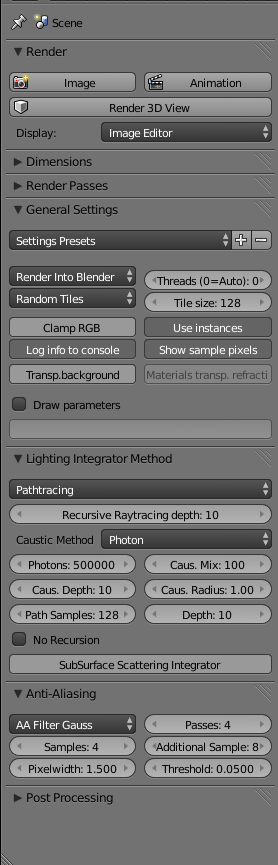
\includegraphics[width=.28\textwidth]{images/generalscreen.png}
    \caption{View of the TheBounty render settings window in Blender, May 2015.}
\end{wrapfigure}

\bigskip

Ray tracing is a rendering technique for generating an image by tracing the path of light through the 3D scene. This technique reproduces the natural behaviour of light and its particular effects on surfaces, such as reflection and refraction, caustics and indirect lighting between diffuse surfaces.

TheBounty usually works as add-on or plugin to a 3D software to provide raytracing capabilities on demand, although it can work as a stand-alone program as well. Blender 3D is the main host application of TheBounty at the moment but there are always on-going projects to add TheBounty support on other 3D packages and modellers.

TheBounty integration in Blender is fairly complete and stable but it should be always considered as a work in progress as Blender and TheBounty keep on evolving. 
}

\section*{TheBounty Renderer features overview}
 \addcontentsline{toc}{section}{TheBounty Renderer features overview}

\paragraph{Lights}
TheBounty supports several types of light sources, i.e. \textit{point}, \textit{spot}, \textit{area} (a rectangular or parallelogram), \textit{mesh} light (which uses a triangle mesh), \textit{sphere} light, \textit{directional} light, \textit{sun} light and \textit{environment}/background light (with importance sampling for efficient image-based lighting, even without global illumination). For more information about the light types, please refer to \tbrref{sec:lights}.

\paragraph{Materials} TheBounty supports \textit{multiple materials} for a single mesh. Materials can consist of different types of materials (diffuse with specular reflection, transparency and translucency)

\todo{Rework this paragraph. This list is really aweful}


\begin{itemize}
\item Multiple materials for a mesh.
\item basic diffuse w. specular reflection, transparency and translucency, support for shader nodes on various properties
\item diffuse+glossy material (Ashikhmin and Shirley), Blinn or anisotropic microfacet distribution w. fresnel effect
\item shader nodes support on diffuse+glossy color, glossiness and bump
\item coated version of the above mentioned, adding specular reflection with fresnel effect (dielectric)
\item basic glass (dielectric) material, with fresnel, filter, absorption and dispersion.
\item emit material
\item export of blender's texture layers as shader nodes
\item blend material, using a blend value or a texture map.
\item subsurface scattering
\end{itemize}

For more information about the different Material options, please refer to \tbrchapref{chapter:materials}.

\paragraph{Textures} Several basic image textures can be used (supported formats are tga, jpeg, png, and even exr and hdr). Also some procedural textures are supported (cloud, marble, wood, voronoi, musgrave, distorted     noise and ``RGB-cube").

For mapping textures to meshes, TheBounty supports multiple textures for a shader, UV coordinates, flat, cube, tube, sphere in global and relative coordinates, blending modes and stencil.  

For more information on this topic, please refer to \tbrchapref{chapter:textureinput}

\paragraph{Backgrounds} TheBounty supports multiple types of backgrounds: single color, two versions of a sunsky (from which the second version has a Night mode), texture and image based lighting and a simple gradient. For more information on this topic, please refer to \tbrref{chapter:backgroundsettings}

\paragraph{Cameras} Different types and settings for camera's can be chosen; a \textit{perspective} camera with raytraced DOF, an \textit{architect} camera with raytraced DOF, an \textit{orthographic} camera and an \textit{angular} camera. For a description and usage of the different camera types, cfr. \tbrref{sec:camerasettings}

\paragraph{Lighting methods} TheBounty gives access to different raytracing lighting methods; direct lighting with support for ambient occlusion and caustic photon maps, path tracing, photon mapping with final gather, bi-directional path tracing and stochastic progressive photon mapping (SPPM).

\paragraph{Volumetrics} TheBounty is able to raytrace volumes, like smoke or clouds. For more information refer to \tbrchapref{chapter:volumetrics}

\paragraph{Adaptive antialiasing} TheBounty supports adaptive (simple color threshold based) antialiasing using variable size reconstruction filters (box, gauss and mitchell-netravali).

\paragraph{Other features} TheBounty also has support for Transparent shadows, multithreaded rendering passes, multipass rendering, radiance map creation. It also has an exporter for XML files (using libXML) for scenes (see YafaRayXML for specifications) and TheBounty is completely plugin based.

\section*{Project History}
 \addcontentsline{toc}{section}{Project History}
The \textit{YafRay} (``Yet Another Free Raytracer'') project was created in 2001 by Alejandro Conty Estévez, and the first public release was in July 2002. These are Jandro's recollections from those years:

\begin{quotation}
\textbf{YafRay}

Introduction

Relevant to Blender v2.31

by Alejandro Conty Estevez,

By the time I started working with YafRay, I was checking out some blender exporters like BMRT and Lightflow. While I was writing some exporting and shading code, I began to be interested in how a raytracer could be written. So when the exams season was in full swing, I became bored (as weird as it may sound) and began to write the main program structure. Once I got a few test renders, I put it off for a year, till the next summer. Then, I wrote the XML loader and YafRay, called "noname" by that moment, began to be an usable program.

Alfredo joined the development almost at the same time. That was of great help. A month later a lot of necessary stuff, like acceleration, were finished and Alfredo ported a lot of his code to YafRay. As the famous hemilight.

Then Luis Fernando Ruiz, a friend of mine and classmate joined to give us a good web site. So we said good bye to that boring plain text web site. We also had the chance to see YafRay rendering on several computers concurrently when Luciano Campal wrote his hack to make YafRay able to work in a distributed way thanks to mosix. It was very exciting when we got access to a 20 computers room for testing. Things started to look very promising when Andrea came with Yable. An experimental export script for an experimental renderer that resulted in a very long thread of cool images at elYsiun. We saw the first nice images done with Blender and rendered with YafRay thanks to him.

We didn't expect that boom. Neither Alfredo nor me. Of course it was the cool export script what was catching people, exporting easily from Blender to a raytracer. We got very excited with all that support from the community. I still get impressed by what people can do with a simple tool like this.

Now more people are getting involved and helping. We begin to have a good documentation section and resources, most of which have been written by Chris Williamson. Basically, it's what you'll see in this chapter. But he is not the only one. YafRay is also getting very easy to use from Blender thanks to Johnny Matthews. I think he spends almost every minute writing Extractor: a new export script for blender. It makes the exporting much more easy by getting all the data directly from blender with nearly no user interaction.

The current power of Extractor and its fast development point out that this could be the future official export scheme for exporting from blender. Anyway, efforts are being made to write a built-in exporter in blender. Alfredo contributed with a lot of shading compatibility code and did some experiments. So it seems we will be able to compare both python and built-in solutions at some point.

YafRay started as an experiment and still is. It's not finished and lacks a lot of features if you compare it with other render engines. I always think is not good enough and that it is hard to imagine what do people see in it. Since people like it for some reason, we now want to really convert it into a full rendering engine that deserves to be called "renderer". This will take some time to have fun coding. We want to add what YafRay lacks (particles, effects, etc...) and to improve global illumination. But only Alfredo De Greef and me are coding YafRay right now, so in order to keep the development up to an acceptable rate, we should get more people to code, more developers. I hope this happens sooner or later.

Finally, I want to thank all the Blender community that supported this project. All those beautiful pictures are what really bring people to YafRay. Likewise, thanks to all the people who give ideas and thoughts on the forums to improve YafRay, and to Juan David G. Cobas for his very appreciated math support.
\begin{flushright}
by \textit{Alejandro Conty Estevez, Chris Williamson, Johnny Matthews}
\end{flushright}
\end{quotation}

By request from the Blender Community, YafRay was added as a Blender plugin from the 2.34 release on, in August 2004. Alejandro de Greef (eeshlo) coded most of the features in the late YafRay releases. At that time it was already evident that a code refactor was necessary in order to add new advanced features to YafRay. The last YafRay release was the 0.0.9 version in Summer 2006.

\begin{wrapfigure}{l}{0pt}
    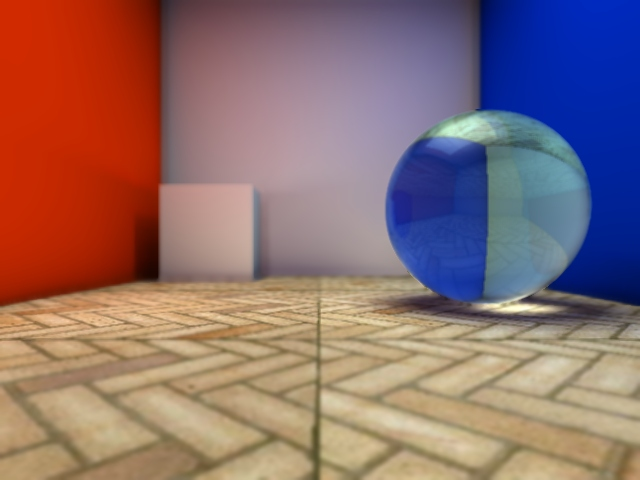
\includegraphics[width=.5\textwidth]{images/caurad_test.jpg}
    \caption{One of the first YafRay renders by \textbf{Jandro}, circa 2001}
\end{wrapfigure}

\textit{YafaRay} is the result of rewriting the YafRay source code from scratch. Mathias Wein (Lynx) started to work on the new engine in December 2005. As a result of the rewriting and to make people aware that it was actually a completely new engine, the YafRay name was changed into YafaRay. Nobody knows for sure what the added 'a' stands for.

\begin{wrapfigure}{r}{0pt}
    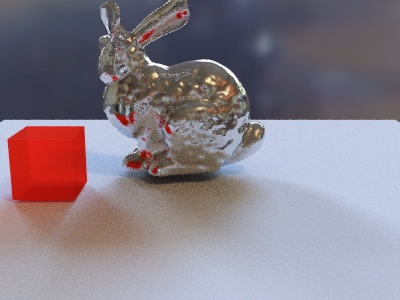
\includegraphics[width=.5\textwidth]{images/bunny_ibl.jpg}
    \caption{One of the first YafaRay renders by \textbf{Lyxn3D}, circa 2005}
\end{wrapfigure}

\bigskip

\textit{TheBounty Renderer} was started by povmaniaco and supported by others when the YafaRay project seemed to start lacking development in 2014. The main objectives of this project are continuing the support for newer Blender versions, optimization and finishing and improving the subsurface scattering.
